% Enable warnings about problematic code
\RequirePackage[l2tabu, orthodox]{nag}

\documentclass{resources/WeSTassignment}
\usepackage{tabularx}
\usepackage{booktabs}
\usepackage[utf8]{inputenc}
\usepackage{amsmath}
\usepackage{graphics}
\usepackage{graphicx}
\usepackage{changebar}
\usepackage{latexsym}
\usepackage{stmaryrd}
\usepackage{booktabs}
\usepackage{amsmath}
\usepackage{wasysym}
\usepackage[export]{adjustbox}
\usepackage[thinlines]{easytable}
\usepackage{framed}
\usepackage{color}
\usepackage{footnote}
\usepackage{listings}
\usepackage{framed}
\usepackage{tikz}

%\solutiontrue
% The lecture title, e.g. "Web Information Retrieval".
\lecture{Introduction to Web Science}
% The names of the lecturer and the instructor(s)
\author{%
  PD Dr. Matthias~Thimm\\{\normalsize\mailto{thimm@uni-koblenz.de}} \and
  Ipek Baris Schlicht\\{\normalsize\mailto{ibaris@uni-koblenz.de}} \and
  Kenneth Skiba\\{\normalsize\mailto{kennethskiba@uni-koblenz.de}}
}
% Assignment number.
\assignmentnumber{2}
% Institute of lecture.
\institute{%
  Institute of Web Science and Technologies\\%
  Department of Computer Science\\%
  University of Koblenz-Landau%
}
% Date until students should submit their solutions.
\datesubmission{24.11.2020, CEST 23:59}

% Specify bib file location.
\addbibresource{bibliography.bib}

\begin{document}

\maketitle

\section{Frame Check Sequence \hfill{24 points}}
\subsection{Checksum \hfill{11 points}}
Calculate the \emph{checksum} of the hexadecimal message \texttt{ab35 c3d1 5231 30ed} using the steps described in Chapters 3.3.2 and 5.2.2 in the textbook \emph{Computer networking: A top-down approach} from Kurose and Ross \footnote{Computer networking: A top-down approach; \emph{James F. Kurose and Keith W. Ross}; 6th Edition; \emph{Pearson Education India}; 2013}. How does the send messages looks like? 

Please write down every calculation step.

\subsection{Cyclic Redundancy Check \hfill{13 points}}
Calculate the \emph{CRC} bits using the \emph{CRC} algorithm, as described in Chapter 5.2.3 in the textbook \emph{Computer networking: A top-down approach} from Kurose and Ross $^1$  for the data \texttt{D= 10001110} and the generator \texttt{g = 1010}. How does the send messages looks like? 

Please write down every calculation step.


\section{Python Programming \hfill{25 points}}
\subsection{Checksum \hfill{15 points} \label{checksum}}
Write a method that computes and returns the checksum of a message. The input message contains four segments and each segment represents a 8-bit binary data.
\begin{enumerate}
    \item In the method, make sure that each step is printed out in the console. For example:
    \begin{lstlisting}
    check_sum = calculate_checksum(message)
    console >> var 1 00000000
               var 2 10011001
               sum   10011001
               ...
               checksum 10001001
    \end{lstlisting}
    
    \item Fill out the following table with the checksum values that are computed by the method.
    \begin{table}[ht]
        \centering
        \begin{tabular}{ll}
             \textbf{Messages} & \textbf{Checksum} \\
             \hline
             \texttt{[0b01101001,0b00100000,0b01101100,0b01101111]} &  \\
             \texttt{[0b01110110,0b01100101,0b00100000,0b01110111]} &  \\
             \texttt{[0b01100101,0b01100010,0b00100000,0b01110011] } &  \\
        \end{tabular}
        \caption{Inputs for the checksum method}
        \label{tab:my_label}
    \end{table}
    
    \item Write another method that validates or rejects given data and checksum. For the corrupted data, the method should output an error message.
    
    \begin{lstlisting}
    validate_data(message, check_sum)
    console >> Corrupted data
    \end{lstlisting}
    
\end{enumerate}
\subsection{TCP Client Server\hfill{10 points}}
In this task you will simulate the checksum operation. You will write a sender (\texttt{sender.py}) and a receiver (\texttt{receiver.py}). The communication between them will be with IPv4 and TCP.  

\begin{enumerate}
    \item \texttt{sender.py} generates random messages as shown Table~\ref{tab:my_label}. When it gets four segments of messages, it calculates the checksum of a message with the method you will implement for Assignment~\ref{checksum} and send them to the receiver.
    \item The \texttt{receiver.py} performs checksum validation with the method you will implement for Assignment~\ref{checksum} and sends the result of the validation to the sender. 
    \item When you execute \texttt{python receiver.py} from the console, you should print out the flow of receiver similarly:
    \begin{lstlisting}
    Connection from ('$SERVER$:$PORT$).
    Got the following message [219, 118, 233, 178] and 17 as
    checksum from the sender
    var 1  00000000
    var 2  11011011
      sum 11011011
    var 1  11011011
    var 2  01110110
      sum 01010010
    var 1  01010010
    var 2  11101001
      sum 00111100
    var 1  00111100
    var 2  10110010
      sum 11101110
    Got the following sum 11111111 after the validation
    ...
    \end{lstlisting}
    
    \item When you execute \texttt{python sender.py} from the console, you should print out the flow of sender similarly:
    
    \begin{lstlisting}
    connected to tmps-$SERVER$:$PORT$
    var 1  00000000
    var 2  11011011
      sum 11011011
    var 1  11011011
    var 2  01110110
      sum 01010010
    var 1  01010010
    var 2  11101001
      sum 00111100
    var 1  00111100
    var 2  10110010
      sum 11101110
  checksum 00010001
Response from the receiver b'Receiver Message: 
Data is correctly received and checksum is 00010001'
...
    \end{lstlisting}

\end{enumerate}


For the programming tasks, you can use the following libraries: \textcolor{red}{\texttt{pickle}}, \textcolor{red}{\texttt{random}}, \textcolor{red}{\texttt{socket}}. Make sure that the messages between sender and receiver are properly printed.

Along with your code, send the print screens of the terminals. 

\section{IPV4 and TCP\hfill{6 points}}
1a) 0xFF24C630 :  
\begin{itemize}
               \item Not a valid IPv4 address.
               \item IPv4 address are divided into following classes and the network id follows a certain range mentioned below: \\ Class A : Range(0-127)\\ Class B : Range(128-191) \\ Class C : Range(192 - 223) \\ Class D : Range(224 - 239) \\ Class E is reserved .
               \item As the above address does not belong to any class it is an invalid IPv4 address.
            \end{itemize}
1b) 198.33.0.255 :
            \begin{itemize}
			\item Not a valid IPv4 address as it is the Direct Broadcast address
            \item The above address belongs to Class c, where Network id is 27 bits and Host id is 8 bits.
            \item The network id would be 198.33.0.0\\The Broadcast address would be 198.33.0.255 both are not used as computer IP addresses
            \end{itemize}
1c)48.96.258.27 :
            \begin{itemize}
            \item  Not a valid address
            \item IPv4 is a 32-bit address where each octet is 8 bits.
            \item The minimum value is 0 (00000000) and the maximum value is 255 (11111111)
            \item In the above IP address the value of third octet is 258 which is out of the range 0-255. Therefore it is not a valid IP address.
            \end{itemize}
2a) TCP is preferred for video streaming if the speed of transmission is important.
			\begin{itemize}
			\item False Statement
			\item In vedio streaming if few packets are lost during transmission the devices using TCP protocol will then have to wait for the retransmission of those packets before receiving any new data. This is achieved by three-way handshake using SYN and ACK bits.
			\item Therefore buffering of unacknowledged packets causes delay and speed of transmission becomes an issue.
			\item Therefore TCP is not preffered for vedio streaming if the speed of transmission is important
			\end{itemize}
2b) TCP is a reliable and stateless protocol which splits application data into equal
size of the packets.
			\begin{itemize}
			\item False Statement
			\item TCP is not stateless protocol rather it is a stateful protocol.
			\item Because a connection is established between the host and receiver through three-way handshake before transmission of data. Adding to this both the host and the receiver maintain session information till the connection termination.
			\item TCP is reliable as it ensures data deliveres in order not damaged and duplicated 
			\end{itemize}
2c)TCP controls the flow control of the networks having different speed of transmission 
			\begin{itemize}
			\item True statement
			\end{itemize}




\section{Tree way handshake \hfill{12 Points}}
Explain with a few sentences the three steps of the process of a TCP three-way handshake.

\section{DNS \hfill{13 Points}}
For the DNS structure shown in Figure \ref{fig:dns} answer the following questions:
\begin{enumerate}
    \item What is the root?
    \item What are the TLD?
    \item What is the FQDN for the point \emph{west}.
    \item What is the domain of \emph{google}.
    \item What is the zone of \emph{com}.
\end{enumerate}

\begin{figure}[h]
    \centering
   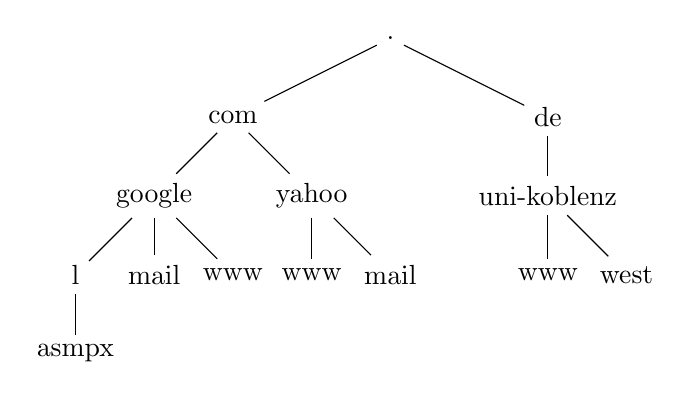
\begin{tikzpicture}
   \node[](root) at (0,0) {.};
   \node[](com) at (-2,-1) {com};
   \node[](de) at (2,-1) {de};
   \node[](google) at (-3,-2) {google};
   \node[](yahoo) at (-1,-2) {yahoo};
   \node[](l) at (-4,-3) {l};
   \node[right of = l](gmail) {mail};
   \node[right of = gmail](gwww) {www};
   \node[right of = gwww](ywww) {www};
   \node[right of = ywww](ymail) {mail};
   \node[below of = de](uni) {uni-koblenz};
   \node[below of = uni](wuni) {www};
   \node[right of = wuni](west) {west};
   \node[below of = l](asmpx) {asmpx};
   
   \draw[-](root) to (com);
   \draw[-](root) to (de);
   \draw[-](com) to (google);
   \draw[-](com) to (yahoo);
   \draw[-](de) to (uni);
   \draw[-](google) to (l);
   \draw[-](l) to (asmpx);
   \draw[-](google) to (gmail);
   \draw[-](google) to (gwww);
   \draw[-](yahoo) to (ywww);
   \draw[-](yahoo) to (ymail);
   \draw[-](uni) to (wuni);
   \draw[-](uni) to (west);
   
   \end{tikzpicture}
   
    \caption{DNS structure}
    \label{fig:dns}
\end{figure}

\end{document}